\documentclass[12pt,a4paper,twoside, openright]{book}
\usepackage[utf8]{inputenc}
\usepackage[T1]{fontenc}
\usepackage[english]{babel}
\usepackage [a4paper,left=3.5cm,bottom=3cm,right=3.5cm,top=3cm]{geometry}
\usepackage{cite}
\usepackage{mathtools}
\usepackage{amssymb}
\usepackage{float}
\usepackage[hidelinks]{hyperref}
\usepackage{listings}
\usepackage[shortcuts]{extdash}
%\usepackage{showframe}
\DeclarePairedDelimiter\ceil{\lceil}{\rceil}

\renewcommand{\baselinestretch}{1.5}
\newenvironment{nopbreak}
  {\par\nobreak\vfil\penalty0\vfilneg\vtop\bgroup}
  {\par\xdef\tpd{\the\prevdepth}\egroup\prevdepth=\tpd}
\usepackage[]{frontespizio}

\newcommand*{\Z}{\mathbb{Z}}
\newcommand*{\N}{\mathbb{N}}

\lstset{
    frame=tb,
    aboveskip=3mm,
    belowskip=3mm,
    basicstyle={\small\ttfamily},
    breaklines=true,
    tabsize=2}

\begin{document}

\begin{frontespizio}
    \Rientro {1.5cm}
    \Margini {1.5cm}{1.5cm}{1.5cm}{1.0cm}
    \Universita {Modena e Reggio Emilia}
%    \Logo [1.5cm]{img/UNIMORE}
    \Facolta {Ingegneria}
    \Corso [Laurea Triennale]{Ingegneria Informatica}
    \Annoaccademico {2019-2020}
    \Titoletto {Prova Finale}
    \Titolo {Modern Cryptography and the HTTPS protocol}
    \Sottotitolo {Crittografia moderna e il protocollo HTTPS}
    \Candidato [118447]{Luca Lumetti}
    \Relatore {Prof. Maurizio Casoni}
    \Correlatore{Dott. Martin Klapez}
\end{frontespizio}

\newpage


\chapter*{\centering {\emph{Introduzione in lingua italiana}}}
\par
In linea con il regolamento della Facoltà di Ingegneria di Modena, ed essendo il seguente elaborato scritto in lingua inglese, la seguente introduzione in lingua italiana sarà una sintesi dell'intero elaborato e sarà l'unica parte scritta in questa lingua. Per una descrizione più esaustiva si faccia riferimento al testo in inglese.
\par
L'obbiettivo di questa tesi è quello di effettuare una panoramica nel campo della crittografia, capirne l'importanza e i campi di applicazione presentando anche alcuni esempi di algoritmi e schemi crittografici moderni. Si conclude infine con la presentazione di un protocollo crittografico, il protocollo HTTPS, oggi ampiamente utilizzato e di notevole importanza.
\par
%introduzione
Viene fatta inizialmente un'introduzione per sottolineare l'importanza della crittografia nel passato, come ad esempio durante la seconda guerra mondiale, e nel presente, con l'avvento dei computer e di internet. Si passa poi a fare una panoramica generale sulla crittografia, introducendo in parte il gergo utilizzato e analizzando i concetti di confidenzialità, integrità e autenticazione. La confidenzialità è la caratteristica di uno schema di generare testi cifrati che, a una entità esterna che non possiede la chiave segreta, non diano alcuna informazione riguardante il messaggio originale. Nella pratica questa definizione viene rilassata e considerata valida solo per avversari efficienti, i quali possono anche avere una probabilità trascurabile, ma non nulla, di ottenere informazioni il messaggio cifrato. Questo rilassamento viene fatto perché il tempo necessario per rompere lo schema è sufficientemente elevato da considerare l'attacco infattibile.\\
 Integrità e autenticazione sono invece due concetti la cui distinzione è abbastanza sfumata e a volte anche messa in discussione. Per entrambi si utilizzano le funzioni di hash, ovvero funzioni deterministiche e unidirezionali. Queste funzioni ricevono in input il messaggio che si vuole spedire e restituiscono una stringa di lunghezza fissata. Dipendentemente dal contesto, l'output di queste funzioni è chiamato \emph{hash del messaggio} oppure \emph{checksum}. Semplificando, il mittente di un messaggio calcola l'hash di questo e lo spedisce insieme al messaggio. Il ricevente ricalcolerà lui stesso l'hash del messaggio ricevuto e lo confronta con l'hash ricevuto per confermarne l'integrità.
\par
%schemi a chiave privata
Nel successivo capitolo vengono presentati i primi schemi crittografici: gli schemi a chiave privata (o simmetrici). Questi schemi hanno la particolarità di utilizzare una singola chiave segreta, sia durante la fase di cifratura, sia durante la fase di decodifica. Per questo motivo la chiave sarà confidenziale esclusivamente tra le due parti coinvolte nella comunicazione. Esistono diversi metodi per costruire schemi a chiave privata, uno di questi è attraverso l'uso di reti a sostituzione e permutazione. Per l'integrità e l'autenticazione, negli schemi a chiave privata si fa uso dei message authentication codes (MAC), costruiti utilizzando le sopracitate funzioni di hash. Vengono infine mostrate le costruzione di uno schema a chiave privata, AES, e di un MAC, HMAC.
\par
%schemi a chiave pubblica
Nel capitolo 4 vengono presentati gli schemi a chiave pubblica (o asimmetrici). Il capitolo comincia con una sezione dedicata a una introduzione riguardate la matematica modulare e la teoria dei gruppi, entrambi alla base della costruzione degli schemi a chiave pubblica. Successivamente si introduce il problema di RSA e la costruzione dell'omonimo schema asimmetrico in una delle sue forme più semplici. Infinite viene mostrata la controparte dei MAC negli schemi a chiave privata, ovvero le firme digitali, utilizzate per associare a una chiave pubblica l'identità di una persona o una qualsiasi entità.
\par
%https
Infine nel quinto capitolo, viene presentato un protocollo che fa uso sia di schemi a chiave pubblica, sia schemi a chiave privata. I primi sono utilizzati per instaurare la comunicazione e scambiarsi la chiave segreta utilizzata poi con lo schema a chiave privata. Questa combinazione di schemi, detta \emph{ibrida}, viene utilizzata perché gli schemi simmetrici sono molto più efficienti della loro controparte. Il protocollo presentato è HTTPS ed è oggi il principale protocollo usato per la comunicazione tra web browsers e web servers. Si è scelto questo protocollo perché, tra i vari schemi usati, sono spesso presenti sia RSA sia AES. Inoltre la verifica dell'autenticità di un sito web, avviene proprio attraverso le firme digitali, attraverso l'uso di varie infrastrutture dette certificates authorities.


\tableofcontents
\listoffigures
%\listoftables

\chapter{Introduction}


\chapter{Cryptography Overview}
Cryptography is the study of using digital coding to secure data accessed. In other words to ensure that data can only be access by authorized entities.\\
To define cryptography jargon we introduce a situation where an entity Alice wants to send a message to another entity Bob through a communication channel. Cryptography is relevant when there's an adversary that tries to access the data sent through the channel without legitimate authorization.\\
The \emph{plaintext} is the message that Alice wants to send to Bob. The \emph{ciphertext} is the data that goes through the channel and one of the resources that an adversary can access.
The process of converting the plaintext to the ciphertext is called \emph{encryption} while the process to convert the ciphertext to the plaintext is called \emph{decryption}.
Encryption and decryption are defined by the \emph{cryptographic scheme}, a set of algorithms that Alice and Bob decide to use before the actual communication, and one or more \emph{keys}, that can be confidential and shared only between the authorized entities or they can also be public depending on the type of scheme used.\\
Regardless of the scheme's type used, which will be discussed later in detail, there are three main features that a cryptographic scheme should have to be defined secure: \emph{confidentiality}, \emph{integrity} and \emph{authentication}.

\section{Confidentiality}
Confidentiality assures that, in a communication, an adversary is unable to obtain any information about the messages exchanged or the key used to encrypt them. This means that the ciphertext should appear to the adversary as completely random bits.
\subsection{Perfectly Secret}
We denote with $\mathcal{M}$, $\mathcal{K}$, $\mathcal{C}$ the message space, key space, and ciphertext space, respectively,  with $\mathsf{Pr}[M = m]$ the probability that the message sent is $m$ and with $\mathsf{Pr}[C = c]$ the probability that the ciphertext is $c$.\\
We can define a cryptographic scheme to be perfectly secret if for every $m \in \mathcal{M}$, every $k \in \mathcal{K}$:
$$
    \mathsf{Pr}[M = m \, | \, C = c] = \mathsf{Pr}[M = m]
$$
This means that the distribution over $\mathcal{M}$ is independent of the distribution over $\mathcal{C}$.
To achieve this definition, the key space $\mathcal{K}$ must be greater than the message space $\mathcal{M}$. This can be impractical and inconvenient because perfect secrecy is defined against an adversary with unbounded computational power. We can relax this latter constraint to be secure against polynomial-time algorithms.

\subsection{Computationally Secret}
Computational security is the aim of most modern cryptographic schemes. Modern encryption schemes can be broken given enough time and computation, nevertheless, the time required even for the most powerful supercomputer today built is in the order of hundreds of years.\\
From the previous definition of perfect secrecy, we add two relaxations:
\begin{itemize}
    \item{Security is only preserved against efficient adversaries.}
    \item{Adversaries can potentially succeed with a negligible probability.}
\end{itemize}
With the term efficient, we refer to an algorithm that can be carried out in \emph{probabilistic polynomial time} (PPT). An algorithm $\mathit{A}$ is said to run in polynomial time, if there exists a polynomial $p(\cdot)$ such that for every $x \in \{0, 1\}^*$, $\mathit{A}(x)$ terminates within at most $p(|x|)$. A probabilistic algorithm is one that has access to some randomness so its results depend on changes.\\
With negligible probability, we refer to a probability asymptotically smaller than the inverse of every polynomial $p(\cdot)$.
So, a function $f(\cdot)$ is $\mathsf{negligible}$ (typically denoted with $\mathsf{negl}$) if for every polynomial $p(\cdot)$ there exists an $N$ such that for all integers $n > N$ it holds that $f(n) < \frac{1}{p(n)}$.

    \subsection{Types of Attack}
    Based on the capableness of the adversary, we can define different types of attack that can be carried out against a scheme, which are:
    \begin{itemize}
        \item{\textbf{Ciphertext-only attack:} is the case when the attacker can only access the ciphertext and try to determine the plaintext that was encrypted. In this case, the attacker is also called "eavesdropper".}
        \item{\textbf{Known-plaintext attack:} in this attack, the adversary learns one or more pairs of plaintexts/ciphertexts encrypted under the same key. The objective of the attacker is to determine the corresponding plaintext of a ciphertext that has not been known yet.}
        \item{\textbf{Chosen-plaintext attack (CPA):} the adversary can obtain the encryption of any plaintext of his choice. Again, the adversary aims to decrypt a ciphertext to get the relative plaintext.}
        \item{\textbf{Chosen-ciphertext attack (CCA):} the final and stronger type of attack. Here the adversary can to encrypt any plaintext and decrypt any ciphertext of its choice. Once again the aim is the same as the previous attacks, but with the constraint that the ciphertext that it wants to crack can't be directly decrypted.}
    \end{itemize}
In both CPA and CCA, the adversary is able to obtain the encryption or the decryption of any message of his choice by using an \emph{oracle}, a black-box that output the requested operations over a message of his choice.

\section{Integrity}
Integrity assures to the receiver that a message is not corrupted or that an adversary modifies and relays it (for example in a man-in-the-middle attack).\\
The decryption of the message is not always needed to modify it but can be enough to have the ciphertext.\\
Hash functions are used to assure the integrity of a message.

\subsection{Hash Functions}
In general, hash functions are just functions that take arbitrary-length strings and compress them into shorter strings.
A hash function is a pair $(\mathsf{Gen}, \mathsf{H})$ such that:
\begin{itemize}
    \item{$\mathsf{Gen}$: is a randomized algorithm that takes as input a security parameter $n$ and outputs a key $s$}
    \item{$\mathsf{H}$: is a deterministic polynomial-time algorithm that takes as input a string $x \in \{0,1\}^*$ and a key $s$ to outputs a string $\mathsf{H}^s(x) \in \{0,1\}^{\mathit{l}(n)}$ where $\mathit{l}$ is a polynomial.}
\end{itemize}
In practice, hash functions are unkeyed, or rather it is included in the function itself.\\
As an example of use of hash functions, imagine that a user A want to send a message $m$ to an user B and he also want to assure its integrity. After they both agree on the hash function to use, A send $(m, \mathsf{H}(m))$, then upon receiving the pair, B itself calculate $\mathsf{H}(m)$ and verify that it is the same it received from A. If they match, $m$ can be considered intact.\\
The domain of $\mathsf{H}$ is unlimited, instead, its image is limited. For the pigeon-hole principles this means that there are infinite pairs of differents string $x$ and $x'$ such that $\mathsf{H}(x) = \mathsf{H}(x')$, this is also known as a \emph{collision}.

\subsection{Collision-resistant hash functions}
Hash functions used in cryptography are also called collision-resistant hash function, to emphatize the importance to have the property that no polynomial-time adversary can find them in a reasonable time.
There are 3 levels of security:
\begin{enumerate}
    \item{\textbf{Collision resistance:} is the most secure level and implies that, given the key $s$, is infeasible to find two different values $x$ and $x'$ such that $\mathsf{H}^s(x) = \mathsf{H}^s(x')$.}
    \item{\textbf{Second preimage resistance:} implies that, given $s$ and a string $x$, is infeasible for a polynomial-time algorithm to find a string $x'$ such that it collide with $x$}
    \item{\textbf{Preimage resistance:} implies that given the key $s$ and an hash $y$, is infeasible for a polynomial-time algorithm to find a value $x$ such that $\mathsf{H}^s(x) = y$.}
\end{enumerate}
Notice that every hash function that is collision resistant is second preimage resistant, also a second preimage resistant function is a preimage resistant function.\\

\subsection{Birthday Attack}
The probability of finding a collision by guessing two random string is inversely proportional to the number of bit outputted by the hash function. For example, SHA-256 has a 256-bit hash output resulting in $2^{256}$ possible results.\\
Now assume we have are given an hash function $\mathsf{H}^s : {0,1}^{*} \rightarrow {0,1}^{l(n)}$. Then we choose at random $q$ distinct strins $x_1,...,x_q$ and compute $y_i := \mathsf{H}^s(x_i)$, $\forall i \in {1,...,q}$. If $q \leq 2^{l(n)}$ the probability is:
$$
    1 - \prod_{i = 1}^{q-1} (1 - \frac{i}{2^{l(n)}})
$$
This problem has been extensively studied and is related to the so-colled birthday problem and an approximation of the above formula is:
$$
    \frac{q^2}{2\cdot2^{l(n)}}
$$
If we want to know how much $q$ are needed to have a probability at least of $50\%$ :
$$
    \frac{q^2}{2\cdot2^{ln(n)}} = 0.5
    \quad \implies \quad
    q = \sqrt{2^{ln(n)}}
$$
This mean that if the output length of a hash function is $l(n)$ bits then the birthday attack finds a collision in $\mathcal{O}(q) = \mathcal{O}(2^{l(n)})$ time.\\

\section{Authentication}
In a cryptographic scheme, authentication is needed to authenticate the entities involved in the comunication. In other words, authentication assure that messages received by Bob are for sure from Alice.\\
To ensure authentication hash functions are used and that's why, in general, authentication imply integrity (but the opposite is not true).

% Even if we have defined hash functions as functions with an infinite domain, in practice they are first constructed to be \emph{fixed-length}, that means their domain is finite, then they are extended to cover the full domain ${0,1}^{*}$.\\
% This extension is made easy by the Merkle-Damg\r{a}rd transform which also preserve the collision resistant propriety.\\
% We will denote the given fixed-length collision-resistant hash function (or \emph{compression function}) by $\mathsf{Gen}_h, h)$ and use it to construct a general collision-resistant hash function $(\mathsf{Gen}, H)$ that maps inputs of any length to outputs of length $l(n)$.\\
% Let $\mathsf{Gen}_h, h)$ be a fixed-length hash function with input length $2l(n)$ and output $l(n)$. Construct a variable-length hash function $(\mathsf{Gen}, H)$ as follow:
% \begin{itemize}
%     \item{$\mathsf{Gen}(n)$: upon input $n$, run the key-generation algorithm $\mathsf{Gen}_h$. $s \leftarrow \mathsf{Gen}_h$.}
%     \item{$H^s(x)$: upon input key $s$ and message $x \in {0, 1}^{*}$, compute as follows:
%         \begin{enumerate}
%             \item{Pad $x$ with zeroes until it's length is a multiple of $l(n)$. Let $L = |x|$ (length of the string) and let $B = \ceil[\Big]{\frac{L}{l(n)}}$ (number of blocks of length $l(n)$).}
%             \item{Define $z_0 := 0^{l(n)}$ and then $\forall i = 1,...,B$, compute:
%                 $$
%                     z_i := h^s(z_{i-1}||x_i)
%                 $$
%                 where $h^s$ is the given fixed-length hash function.}
%             \item{Output $z = H^s(z_B||L)$.}
%         \end{enumerate}}
% \end{itemize}
% We remark that the value $z_0$, also known as \emph{IV} or \emph{initialization vector} can be replaced with any costant of length $l(n)$ bits.

% \subsection{Message Authentication Code (MAC)}
% A message authentication codes, also know as \emph{tags}, are small string used to authenticate a message and to protect its integrity


\chapter{Private Key Cryptography}
With \emph{private-key cryptography} we refer to schemes that use a single key to encrypt and decrypt a message, for this reason, we will refer to them as \emph{symmetric} schemes.
A \textbf{private-key scheme} is a tuple $(\mathsf{Gen}, \mathsf{Enc}, \mathsf{Dec})$ such that:
\begin{itemize}
    \item{\textbf{$\mathsf{Gen}(\cdot)$:} is a randomized polynomial algorithm that generates the key. It takes as input a security parameter $n$ and outputs a key $k$ that satisfies $|k| \geq n$.\\
        We will write this as $k \leftarrow \mathsf{Gen}(1^n)$.}
    \item{\textbf{$\mathsf{Enc}(\cdot)$:} is a probabilistic polynomial-time algorithm that encrypts the message (or other forms of information) to send. It takes as input a key $k$ and a message $m$ to output a ciphertext $c$. We will refer to the unencrypted message also as plaintext.\\
        We will write this as $c \leftarrow \mathsf{Enc}_k(m)$.}
    \item{\textbf{$\mathsf{Dec}(\cdot)$:} is a deterministic polynomial-time algorithm that takes as input a ciphertext $c$ and a key $k$, and outputs a plaintext $m$.\\
        We will write this as $m := \mathsf{Dec}_k(c)$}
\end{itemize}
It's also required that for every $n$, every $k$ and every $m$ it holds that $m = \mathsf{Dec}_k(\mathsf{Enc}_k(m))$.\\
Now we want to look which tools are used in the construction of secure private-key scheme.

\section{Pseudorandom Permutations}
Pseudorandom functions are functions that map n-bits strings to n-bit strings and that cannot be distinguished from a random permutation chosen, uniformly, from every function that map n-bit string to n-bit string.
The first set of function, for a key of length $s$ bit, have a cardinality of $2^{s}$, while the second set has a cardinality of $2^{n\cdot2^n}$.\par
Pseudorandom permutations are pseudorandom functions with some extra proprieties:
Let $F : \{0,1\}^{n} \times \{0,1\}^{s} \rightarrow \{0,1\}^{n}$ be an efficient, length-preserving, keyed function and $F_k(m) := F(m, k)$.
$F$ is a pseudorandom permutation (PRP) if:
\begin{itemize}
    \item{$\forall k \in \{0,1\}^{s}$, $F$ is a bijection from $\{0,1\}^{n}$ to $\{0,1\}^{n}$}.
    \item{$\forall k \in \{0,1\}^{s}$ exists an efficient algorithm $F^{-1}_k$.}
    \item{For all probabilistic polynomial-time distinguishers $D$:
        $$
            |\mathsf{Pr}[D^{F_k}(n) = 1] - \mathsf{Pr}[D^{f_n}(n) = 1]| < \mathsf{negl}(n)
        $$
        where $k$ is chosen uniformly at random from $\{0,1\}^{s}$ and $f_n$ is chosen uniformly at random from the set of every permutations on n-bit strings.
        }
\end{itemize}


\section{Block Ciphers}
\par
Block ciphers are PRPs families that operate on a block of a fixed length. To ensure security against CPA, there are various modes of operation for block ciphers, like \emph{Electronic Code Block} (ECB), \emph{Cipher Block Chaining} (CBC), and \emph{Counter Mode} (CTR).

\subsection{Electronic Code Block}
\par
Given a plaintext $m = m_1,...,m_l$, the encryption is obtained by encrypting each block separately: $c = \langle F_k(m_1),...,F_k(m_l) \rangle$.
The decryption is carried out by applying to every block $F_k^{-1}$. Since the encryption process is deterministic, repeated blocks will be repeated also in the ciphertext. This means that this mode is not CPA-secure neither has indistinguishable encryption in the presence of an eavesdropper.
\begin{figure}[H]
    \centering
    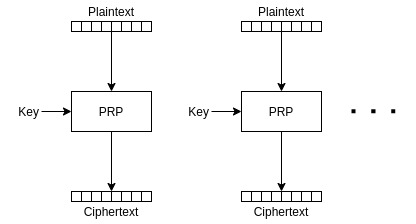
\includegraphics[width=0.6\textwidth]{img/private-key/ecb.jpg}
    \caption{ECB encryption.}
\end{figure}

\subsection{Cipher Block Chaining}
\par
First an initial vector IV of length n is chosen. Then, is set $c_0 = IV$ and for every $i > 0$, $c_i := F_k(c_{i-1} \oplus m_i)$. The final ciphertext is $<IV,c_1,...,c_l>$. The IV is not kept secret to allow decryption. The encryption of single blocks must be carried out sequentially
\begin{figure}[H]
    \centering
    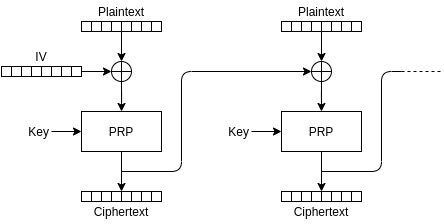
\includegraphics[width=0.6\textwidth]{img/private-key/cbc.jpg}
    \caption{CBC encryption.}
\end{figure}

\subsection{Randomized Counter Mode}
\par
As in CBC, an IV of length n is chosen. Then is computed $r_i := F_k((IV + i)\;\mathsf{mod}\;2^n)$. Then each block of the plaintext is computed as $c_i := r_i \oplus m_i$. Unlike in CBC, with CTR it's possible to encrypt and decrypt in parallel.
\begin{figure}[H]
    \centering
    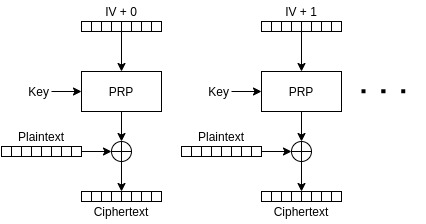
\includegraphics[width=0.6\textwidth]{img/private-key/ctr.jpg}
    \caption{CTR encryption.}
\end{figure}

\begin{figure}[h]
    \centering
    \fbox{
\includegraphics[width=0.2\textwidth]{img/private-key/unimore-original.jpg}}
    \fbox{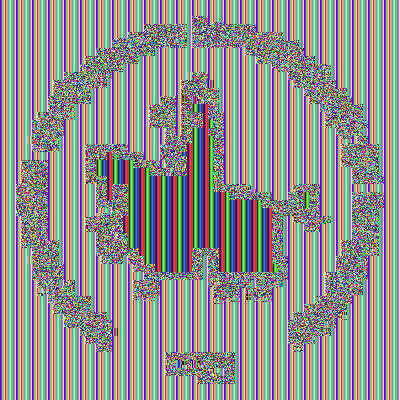
\includegraphics[width=0.2\textwidth]{img/private-key/unimore-ecb.jpg}}
    \fbox{
\includegraphics[width=0.2\textwidth]{img/private-key/unimore-ctr.jpg}}
    \fbox{
\includegraphics[width=0.2\textwidth]{img/private-key/unimore-cbc.jpg}}
    \caption[Comparison of the different encryption modes]{From left to right: original image, image encrypted with ECB, image encrypted with CTR, image encrypted with CBC. It's easy to notice the problem with ECB.}
\end{figure}

% Nel caso volessi presentare DES, cambiare in Feistel Network. Bisognerà in
% qualche modo introdurre le S-boxes
\section{Substitution-Permutation Networks}
\subsection{Confusion-diffusion}
The confusion-diffusion paradigm has been introduced by Shannon for concise construction  pseudorandom functions. The idea is to break the input up into small parts, execute on them different random functions, mixed the outputs together and, repeat the process for a finite amount of time. One cycle of this process is called \emph{round}, while the full construction is called \emph{network}.\\
Shannon's original definitions are that confusion refers to making the relationship between the ciphertext and the key as complex as possible, diffusion refers to hide the relationship between the ciphertext and the plaintext.
Confusion achieves the fact that each bit of the ciphertext depends on several parts of the key. This means that, even if a single bit of the key is changed, most of the bits in the ciphertext will be affected.
Diffusion implies that changing a single bit in the plaintext results in a change of (statistically) half of the bits in the ciphertext. Also, if one bit of the ciphertext is changed, half of the bits of the plaintexts change.

\subsection{Substitution-Permutation Networks}
Substitution-permutation networks are a practical implementation of the confusion-diffusion paradigm. The substitution part is achieved by small random functions called \emph{S-boxes} and the permutation part is achieved by mixing up the outputs of those functions. In the intermediate results, a key is XORed with the output of the round. Different keys are used each round and each key is derived from the previous one (that is called the \emph{master key}).

\section{Advanced Encryption Standard}
AES is a common symmetric key block cipher used worldwide to protect data. It is the successor of \emph{DES} (Data Encryption Standard), another block cipher that now has been classified insecure because of its key length, and after some attacks became too efficient. It has been chosen after a public competition held to meet the need for a new encryption standard.\\
Before introducing the concrete algorithm, we must introduce Galois field, a finite field used during a step of AES.

\subsection{Galois Field}
A Galois Field (or finite field) is a field with a finite number of elements. The most common fields used are given by the integers $\mathsf{mod}\,p$ where $p$ is a prime number, also written as $\mathsf{GF}[p]$. For $n > 1$, with $\mathsf{GF}[p^n]$ we refer to all polynomials of degree $n-1$ with coefficients coming from $\mathsf{GF}[p]$. As an example, $\mathsf{GF}[2^3]$ is a field with $8$ elements (the integers from 0 to 7) and they can all be represented as a polynomial of degree $2$ (6 can be represented as $110_2$ or $x^2+x$).\\
Even if the sum between polynomials is trivial, the multiplication works differently: an irreducible polynomial $g(x)$ of degree $n$ is chosen, then the multiplication in $\mathsf{GF}[p^n]$ is the ordinary product, except you have to take the remainder of the division by $g(x)$. A different $g(x)$ defines a different field.

\subsection{Encryption Method}
The security of AES comes from confusion and diffusion achieved by a substitution\=/permutation network with a block size of 128 bit and it supports three different key lengths: 128, 198, and 256 bits. Every key length uses a different number of rounds, i.e., 10, 12, and 14, respectively.\\
Each block of length 128 bits is rearranged in a 4x4 bytes array, called \emph{state}, and for every round the following steps are executed:
\begin{enumerate}
    \item{\textbf{AddRoundKey:} A 16 byte round key is derived from the master key and it's interpreted as a 4x4 array. Then, the key is XORed with the state array.\\This step consists of computing $a_{i,j} = a_{i,j} \oplus k_{i,j}$ for every $i,j \in {1,...,4}$ where $a_{i,j}$ is the $i^{th}$ row and $j^{th}$ column of the state array and $k_{i,j}$ is the $i^{th}$ row and $j^{th}$ column of the key array.}
    \item{\textbf{SubBytes:} Each byte of the state array is substituted by another byte, according to a single fixed lookup table \emph{S}. So, it consists in computing $a_{i,j} = S(a_{i,j})$.}
    \item{\textbf{ShiftRows:} Each row of the state array is cyclically shifted to the left as follows: the first row of the array is untouched, the second row is shifted one place to the left, the third row is shifted two places to the left, and the fourth row is shifted three places to the left.}
    \item{\textbf{MixColumns:} In this step, each column is mixed via an invertible linear transformation. Specifically, each column is interpreted as a polynomial over $\mathsf{GF}[2^8]$ with $g(x) = x^4 + 1$, and is multiplied with a fixed polynomial $c(x) = 3x^3 + x^2 + x + 2$.}
\end{enumerate}
In the final round, the MixColumns stage is replaced with an additional AddRoundKey step.

\section{Message Authentication Codes}\label{sec:mac}
Everything we have seen until now assures only confidentiality. As introduced in \autoref{chap:overview}, message authentication codes (MAC) also called \emph{tags} are used to introduce both integrity and authentication.\\
Even if an encryption scheme assures confidentiality, integrity, and authentication are important to assure that the message is not tampered by an external entity. This is a property of encryption schemes called \emph{malleability}.\\
For example, in CBC an attacker, because the IV and ciphertext blocks are directly XORed with the next block output, a bit changed in the IV or the ciphertext block corresponds with a bit changed in the plaintext. If the attacker can guess the format of the unencrypted message the attacker could be able to change sensitive information on the plaintext.\\
A message authentication code (MAC) is a tuple of PPT algorithms $(\mathsf{Gen},\mathsf{Mac},\mathsf{Vrfy})$ such that:
\begin{itemize}
    \item{$\mathsf{Gen(\cdot)}$: it takes as input $n$ and outputs a uniformly distributed key of length $n$.\\We will write this as $k \leftarrow \mathsf{Gen}(1^n)$.}
    \item{$\mathsf{Mac_k(\cdot)}$: It receive as input a key $k \in \{0,1\}^n$ and a message $m \in \{0,1\}^{*}$ to output a \emph{tag} $t \in \{0,1\}^{*}$.\\We will write this as $t \leftarrow \mathsf{Mac}_k(m)$.}
    \item{$\mathsf{Vrfy_k(\cdot,\cdot)}$ on input $k \in \{0,1\}^n$, $m \in \{0,1\}^{*}$ and $t \in \{0,1\}^{*}$ it output a bit $b \in {0,1}$.\\We will write this as $b \leftarrow \mathsf{Vrfy}_k(m, t)$.}
\end{itemize}
It also required that for every $n$, every $k$, and every $m$ it holds that:
$$
\mathsf{Vrfy}_k(m, \mathsf{Mac}_k(m)) = 1
$$
The security of MAC is that an adversary can't forge a valid tag for a new message in a reasonable time.\\
The construction of MAC can be based on block ciphers, like \emph{CBC-MAC}, or collision-resistant hash functions built with the Merkle-Damg\r{a}rd transform (see \autoref{sec:collisionresistant} and \autoref{sec:merkledamgard}), like \emph{NMAC} or \emph{HMAC}.

\subsection{HMAC construction}
With $H^s_{\mathsf{IV}}(x)$ the hash function constructed with Merkle-Darmg\r{a}rd transform with $z_0$ set to an arbitrary value $\mathsf{IV}$ and we also define a keyed version of the compression function $h^s(x)$ used in $\mathsf{H}$ by $h^s_k(x) = h^s(k\;||\;x)$. Two constants are also defined: $\mathsf{opad}$ and $\mathsf{ipad}$ of length $n$ (the length of a single block of the input to $\mathsf{H}$).\\
The string $\mathsf{opad}$ is formed by repeating the byte $\mathsf{0x5C}$ as many times needed and the string $\mathsf{ipad}$ is formed in the same way using the byte $\mathsf{0x36}$.\\
The HMAC construction is the same defined above in this section, with two additions:
\begin{itemize}
    \item{The $\mathsf{Gen}$ algorithm also run the key generation for the hash function obtaining the value $s$.}
    \item{The $\mathsf{Mac}_k$ algorithm is computed by:
$$
    \mathsf{HMAC}^s_k(x) = \mathsf{H}^s_\mathsf{IV}(k \oplus \mathsf{opad}\;||\;\mathsf{H}_\mathsf{IV}(k \oplus \mathsf{ipad}\;||\;x))
$$
        }
\end{itemize}
The hash function $\mathsf{H}$ can be any cryptographic hash function like SHA-1, SHA-256, etc..., and the relative HMACs are named HMAC-SHA1, HMAC-SHA256. The cryptographic strength of HMAC depends on the properties of the underlying hash function, so using hash functions like MD5 or SHA-1 is not recomended.
%encrypt then auth


\chapter{Public Key Cryptography}

\chapter{HTTPS - Hypertext Transfer Protocol Secure}
Private and public key schemes as well as digital signatures can be found in many protocols used over the internet to create secure communication channels. One of them is the Hypertext Transfer Protocol Secure (HTTPS), which is the extension of the Hypertext Transfer Protocol (HTTP). It's widely used on the internet in the communication between browsers and web servers. Many reasons rise to the need for a secure protocol, indeed HTTP is vulnerable to eavesdropping, tampering, and other attacks that can be carried out with a MITM. HTTPS assures that a communication between a browser and a website an attacker can't interference.

\section{HTTP}
The Hypertext Transfer Protocol is an application-layer protocol for transmitting hypermedia documents, such as HTML documents. It's often based over the TCP/IP layer and it is stateless. It works in a request/reply fashion, based on the exchange of individual messages. Requests are the messages sent by the client (usually a web browser), responses are messages sent back by the server.
\subsection{Request}
An HTTP request includes:
\begin{itemize}
    \item{\textbf{Method:} specifies the operation that the client wants to execute on the server, like GET, POST, PUT, ...}
    \item{\textbf{URL:} is the identifier of the requested object}
    \item{\textbf{Version:} the HTTP version used}
    \item{\textbf{Headers:} additional information that can be used by the server, like date, the browser used, cookies. They are not mandatory.}
\end{itemize}
Here is an example of an HTTP request:
\begin{lstlisting}
    GET /directory/page.html HTTP/1.1
    Connection: close
    User-agent: Mozilla/5.0 (X11; Linux x86_64)
    Accept: text/html, image/jpeg
    Accept-language: it-IT,en-US
\end{lstlisting}

\subsection{Response}
An HTTP response includes, besides the content of the resource requested, a header with the HTTP version, a status code, and some additional response information.
Here is an example of an HTTP response:
\begin{lstlisting}
    HTTP/1.1 200 OK
    Content-language: it
    Content-length: 18844
    Content-type: text/html; charset=UTF-8
    Date: Mon, 22 Jun 2020 21:50:53 GMT
    Server: nginx

    <!DOCTYPE html><head> ... the page ... </html>
\end{lstlisting}
\subsection{HTTPS vs HTTP}
HTTPS is an extension of HTTP, which means that the request and response format is exactly the same but the messages exchanged are encrypted by a cryptographic protocol. The protocol used is Transport Layer Security (TLS) and is the successor of Secure Socket Layer (SSL), today deprecated. That's why HTTPS is also referred to as HTTP over TLS.\\
Other differences are that HTTPS uses the well-known port 443, while HTTP uses the well-known port 80 and the URL starts with \texttt{https://} instead of \texttt{http://}.

\section{TLS}
The TLS protocol allows to client/server application to communicate while preventing the tampering and eavesdropping of informations. In the HTTPS procol, only the server authenticate to the client but not vice versa. Is the evolution of another protocol called SSL, today marked as insecure and not anymore supported by browser. Even first versions of TLS are planned to be deprecated during 2020. The most recent version of TLS is 1.3.\\
To establish a secure connection, the client and the server, before trasmitting any other informations, perform an \emph{handshake}.
\subsection{Handshake}
TLS handshake occur after a TCP connection has been opened via a TCP handshake. The last ACK sent by the client also contains the first step of the TLS handshake.
\subsubsection{1 - Client Hello}
This is the first step, performed by the client and also know as Cryptographic negotiation. The client share with the server the list of his supported TLS version, his cipher suite and it might send options about the ciphers or client's infos. The client also generate a random 32-byte number, used later to generate symmetric keys, and a session ID used to identify the connection.\\
Example of Client Hello taken using tshark:
\begin{lstlisting}
Handshake Protocol: Client Hello
Length: 510
Version: TLS 1.2 (0x0303)
Random: 55 2a 89 9e f4 21 04 49 f3 17 6a 39 8b cc 4c 39 ab 44 24 3b 25 ce 1b 95 cc 9a 47 52 ac 1c 29 18
Session ID Length: 32
Session ID: 54 33 56 39 b8 5f 27 4d 56 cb b1 0f 45 6a b2 92 e9 8d a2 95 97 bd f9 8d f6 b3 b2 a0 4e 9c 4e 7f
Cipher Suites Length: 32
Cipher Suite: TLS_AES_128_GCM_SHA256
Cipher Suite: TLS_AES_256_GCM_SHA384
... more ciphers ...
Cipher Suite: TLS_RSA_WITH_AES_128_GCM_SHA256
Cipher Suite: TLS_RSA_WITH_AES_256_CBC_SHA256
Extensions Length: 405
... extensions ...
\end{lstlisting}

\subsubsection{2 - Server Hello}
The server reply to the client hello with a server hello. The server send a message containing the TLS server version and a cipher suite, both chosen among the ones received from the Client Hello. It also send a 32-byte random number and the session ID received by the client.\\
Example of Server Hello taken using tshark:
\begin{lstlisting}
Handshake Protocol: Server Hello
Handshake Type: Server Hello (2)
Length: 96
Version: TLS 1.2 (0x0303)
Random: 72 f2 70 6b 47 f1 d5 98 73 20 68 78 7c 26 a3 7d da 54 d8 30 3a 48 8c bf a7 90 68 95 c5 c0 68 97
Session ID Length: 32
Session ID: 54 33 56 39 b8 5f 27 4d 56 cb b1 0f 45 6a b2 92 e9 8d a2 95 97 bd f9 8d f6 b3 b2 a0 4e 9c 4e 7f
Cipher Suite: TLS_ECDHE_RSA_WITH_CHACHA20_POLY1305_SHA256 (0xcca8)
Extensions Length: 24
... extensions ...
\end{lstlisting}

\subsubsection{3 - Server Certificate}
The server send his certificate and his public key to the client to prove his identity.\\
\begin{lstlisting}
Handshake Protocol: Certificate
Handshake Type: Certificate (11)
Length: 2568
Certificates Length: 1174
Certificates (1174 bytes)
Certificate Length: 1174
Certificate: 308204923082... (id-at-commonName=Let's Encrypt Authority X3, id-at-organizationName=Let's Encrypt, id-at-countryName=US)
version: v3 (2)
serialNumber: 0x0a0141420000015385736a0b85eca708
Algorithm Id: 1.2.840.113549.1.1.11 (sha256WithRSAEncryption)
modulus: 0x009cd30cf05ae52e47b7725d3783b3686330ead735261925...
publicExponent: 65537
... more ...
\end{lstlisting}

\subsubsection{4 - Client Key Exchange}
A pre-master secret key is created by the client and sent to the server. How the key is created might depend by the cipher suited selected. The key is encrypted using the server public key. Both client and server compute the \emph{master secret} key using a Pseudorandom function that takes as input the pre-master secret and the 32-byte random value exchanged early. This master key is 48 bytes long and is used to symmetrically encrypt data with one of the private-key cipher chosen from the cipher suite.

\subsubsection{5 - Client Handshake Finished}
The client is now ready to switch to a secure enviroment. From now on every data sent to the server will be encrypted using the symmetric scheme chosen and the master key. The client sent his first encrypted message saying that the handshake for the client is finished.

\subsubsection{6 - Server Handshake Finished}
Also the server is ready to switch to a secure enviroment and from now on every data sent by the server will be encrypted using the same algorithms used by the client. It sent an encrytpted message saying that the handshake for the server is terminated.


\chapter{Conclusions}


\appendix

\nocite{*}
\bibliographystyle{plain}
\bibliography{thesis}

\end{document}
